% !TeX root = ..

\section{
  Классификация оптимизационных задач
  маршрутизации инструмента
  машин фигурной листовой резки с~ЧПУ
}
\label{sect:1.4}
\setcounter{equation}{0}

Существующая  классификация задач маршрутизации инструмента
машин фигурной листовой резки с ЧПУ определяется
типом использованной техники резки и способом задания
возможных точек входа инструмента в контур.
В работе \cite{intro13}
все задачи маршрутизации разбиты на пять основных классов
(см. рис.~\ref{dewil}).

\begin{itemize}
\item Задача непрерывной резки
({\it CCP, Continuous Cutting Problem}):
каждый контур вырезается целиком,
и резка может начаться в любой точке контура (и в ней же завершиться).
Переход к следующему контуру осуществляется на холостом ходу инструмента машины с ЧПУ.

\item Задача коммивояжера
({\it TSP, Traveling Salesman Problem}):
самый простой частный  случай задачи {\it CCP} --
каждый контур вырезается целиком,
и резка может начаться в только в одной заранее определенной точке контура
(и в ней же завершиться).

\item Обобщенная задача коммивояжера
({\it GTSP, Generalized Traveling Salesman Problem}),
также частный случай задачи {\it CCP} --
резка может начаться только в одной из заранее
заданных точек на контуре (их может быть несколько),
контур также должен быть вырезан целиком.

\item Задача резки с конечным набором точек
({\it ECP, Endpoint Cutting Problem}):
резка может начаться только в одной из
заранее заданных точек на контуре,
однако контур может быть вырезан за несколько подходов, по частям.

\item Задача произвольной резки
({\it ICP, Intermittent Cutting Problem})
-- наиболее общая формулировка задачи моделирования траектории резки,
когда не накладывается никаких ограничений на выбор точек начала и конца резки,
а также на последовательность резки контуров и их частей:
контуры могут резаться по частям,
за несколько подходов,
и резка может быть
начата и продолжена в любой точке контура.

\end{itemize}

\begin{figure}[H]
  \centering
  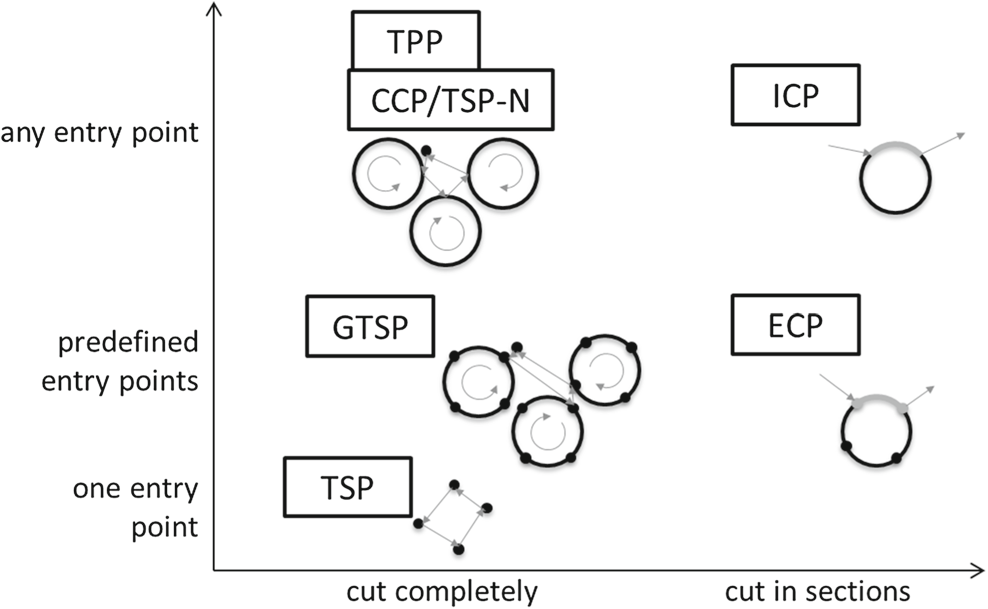
\includegraphics[width=0.9\textwidth]{dewil.png}
  \caption{
    Основные классы задач маршрутизации инструмента
    для машин фигурной листовой резки
    согласно \cite{intro13}
  }
  \label{dewil}
\end{figure}

Обычно предполагается также,
что точки врезки в материал,
которые из-за технологических требований резки
(\ref{pierce-constraint})
не совпадают с точками входа в контур,
однозначно определяются выбранными точками входа в контуры (и наоборот)
и находятся от контуров на фиксированном расстоянии.
Отметим, что число сегментов резки
$K$ в кортеже (\ref{tuple})
$ROUTE \hm = \left<
  M_0, M_1, S_1, M_1^*, M_2, S_2, M_2^*, \,\dots, M_K, S_K, M_K^*,
  i_1, i_2, \,\dots, i_K
\right>
$
для первых трех классов задач маршрутизации всегда равно количеству вырезаемых контуров
$N$.

Введем следующее определение.

\begin{opred}
  \label{def:base-segment}
  {\bf Базовым сегментом резки}
  $B^S$
  для сегмента резки
  $S=MM^*$
  будем называть часть траектории сегмента,
  не содержающую траектории входа в контур
  {\it lead-in} и выхода из контура {\it lead-out},
  т.е.
  \begin{equation}
    S=MM^* = M \, lead_{in} \, B^S \, lead_{out} \, M^*
    .
    \label{base-segment}
  \end{equation}
\end{opred}

Будем полагать,
что базовый сегмент,
в отличие от сегмента резки,
не имеет направления,
но тогда если базовый сегмент содержит
один или более замкнутых контуров,
то при определении сегмента резки $S$
нам необходимо для каждого контура задать направление резки
(<<+>> при резке по часовой стрелке,
<<-->> против часовой).

Таким образом,
каждый базовый сегмент резки
содержит список
$L(B^S)$
своих замкнутых контуров (может быть пустой).
Пусть
$|L(B^S)|$ --
длина этого списка, тогда кортеж $ROUTE$ (\ref{tuple})
в терминах базового сегмента резки запишется в следующем виде:

\begin{multline}
  ROUTE =  \langle
    M_0, M_1 B^{S_1} M_1^* p_1^1 \,\dots, p_1^{|L(B^{S_1})|},
    M_2 B^{S_2} M_2^* p_2^1 \,\dots, p_2^{|L(B^{S_2})|},
    \\ \dots, \\
    M_K B^{S_K} M_K^* p_K^1 \,\dots, p_K^{|L(B^{S_K})|},
    i_1, i_2, \,\dots, i_K
  \rangle
  ,
  \label{tuple-base-segments}
\end{multline}
где $p_t^r=\pm 1$
(указано направление резки в контуре с номером $r$ базового сегмента $B^{S_t}$),
$r=\overline{1, |L(B^{S_t})|}$.

Формула (\ref{tuple-base-segments})
дает наиболее общее формальное описание маршрута резки (траектории интрумента)
машины листовой резки с ЧПУ.

В примере резки двух деталей
на рис.~\ref{cut2-1}
два базовых сегмента изображены пунктирными
линиями
(использована мультиконтурная техника резки).

\begin{figure}[H]
  \centering
  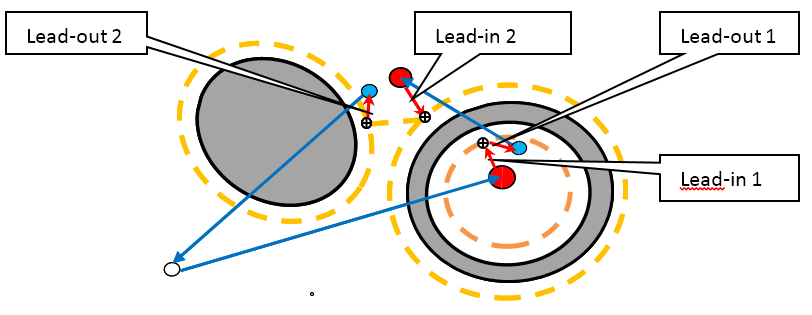
\includegraphics[width=0.9\textwidth]{cut2-1.png}
  \caption{
    Пример схемы резки трех замкнутых контуров
    с использованием двух~сегментов резки
  }
  \label{cut2-1}
\end{figure}

Пример сегмента резки, в котором использована техника совмещенного реза,
и базового сегмента, содержащего четыре контура,
приведен на рис.~\ref{cut4-3}.
Стрелками отмечено направление резки контуров,
цифрой {\it 1} -- точка врезки.

\begin{figure}[H]
  \centering
  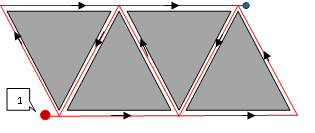
\includegraphics[width=0.7\textwidth]{cut4-3.png}
  \caption{
    Сегмент резки, включающий базовый сегмент
    с использованием техники~резки <<совмещенный рез>>
  }
  \label{cut4-3}
\end{figure}

На основе концепции базового сегмента введем еще
два класса задач маршрутизации инструмента машин
фигурной листовой резки с ЧПУ.

\begin{opred}
  \label{def:SCCP}
  {\it SCCP (Segment Continuous Cutting Problem)}
  --
  задача с фиксированным числом $K$
  сементов резки
  (и базовых сегментов резки
  $B^{S_k}, k \in \overline{1, K}$).
\end{opred}

{\it Замечание}:
Если все граничные контуры деталей
$C_1, C_2 \,\dots, C_N$ --
это базовые сегменты $B^{S_k}, k \in \overline{1,K}$,
и $N=K$,
тогда {\it SCCP} эквивалентна {\it CCP}.

Предположим, что для исходной задачи маршрутизации
определен конечный набор (ансамбль)
базовых сегментов резки размерности $T$.
Этот ансамбль соответствует ансамблю задач
$\{SCCP_i, i \in\overline{1,T}\}$.

\begin{opred}
  {\it GSCCP (Generalized SCCP)} -- есть
  $\{SCCP_i, i \in\overline{1,T}\}$.
\end{opred}

Как нетрудно видеть,
введя классы {\it SCCP} и {\it GSCCP},
мы значительно расширили существующую
классификацию задач маршрутизации инструмента
для машин листовой резки с ЧПУ.
Фактически {\it SCCP} и {\it GSCCP} являются подклассами {\it ICP},
содержащими все задачи с конечным набором базовых сегментов резки,
т. е.
$CCP \subset SCCP \subset GSCCP \subset ICP$.
Таким образом, в классе {\it ICP} выбран большой подкласс
задач маршрутизации,
для которых можно разработать эффективные алгоритмы оптимизации.

На рис.~\ref{x-classify}
приведена расширенная классификация этих задач.
Все классы сгруппированы в три группы,
различающиеся мощностью множеств,
из которых выбираются точки входа в контуры
(точки врезки).

Далее рассмотрим подход,
основанный на  дискретизации трех клаcсов задач маршрутизации
первой группы ({\it CCP, SCCP, GSCCP})
и сведении их к задаче о последовательном обходе мегаполисов,
в которой  используется математическая модель А. Г. Ченцова,
описанная подробно во второй части настоящей монографии
(главы 3--5).

\begin{figure}[H]
  \centering
  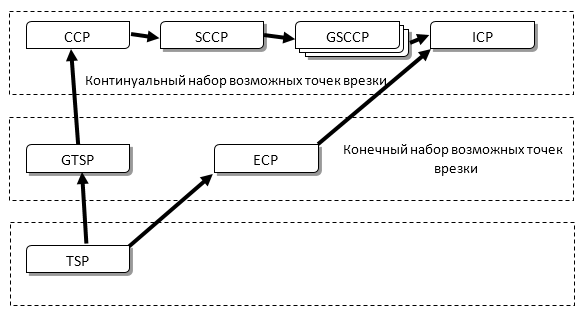
\includegraphics[width=0.9\textwidth]{x-classify.png}
  \caption{
    Расширенная классификация задач
    маршрутизации инструмента машин листовой резки
  }
  \label{x-classify}
\end{figure}

Эта модель может быть интерпретирована
как математическая модель обобщенной задачи коммивояжера ({\it GTSP})
с дополнительными ограничениями.
(Следует различать модель {\it GTSP}
и~задачу маршрутизации {\it GTSP} из второй группы,
которая представляет собой дискретный вариант задачи {\it CCP}).
В отличие от классического {\it GTSP} эта модель
предусматривает учет так называемой внутренней работы
(в данном случае -- процесса резки).
Кроме того, модель мегаполисов с
использованием специальной схемы динамического программирования
учитывает сложные типы целевых функций и сложные ограничения,
в том числе динамические.
Наконец, принимая во внимание ограничения предшествования,
можно получить точные решения для дискретных вариантов {\it SCCP}
достаточно большой размерности.

В качестве примера рассмотрим задачу {\it GSCCP},
которая содержит две
задачи {\it SCCP} с разными наборами сегментов,
показанными на рис.~\ref{gsccp-both},
где а -- 21~базовый сегмент
и б -- 18 базовых сегментов соответственно.

Первый набор базовых сегментов,
(рис.~\ref{gsccp-both}, {\it а})
задан всеми граничными контурами деталей, т. е.
$C_j = B^{S_j}, j\in\overline{1,N}, N=K=21$.
В этом случае мы имеем классическую задачу {\it CCP}.
На рис.~\ref{gsccp-both}, {\it б} восемь
базовых сегментов заданы внешними граничными контурами <<серых>> деталей.
Три дополнительных базовых сегмента заданы шестью
внешними граничными контурами <<цветных>> деталей
(один базовый сегмент состоит из двух внешних контуров плюс перемычка между ними).
Эти контуры будут вырезаться <<цепной>> резкой попарно в одном базовом сегменте.
Наконец, семь базовых сегментов заданы внутренними
граничными контурами всех деталей,
в которых имеются отверстия.
В этом случае мы имеем набор из восемнадцати
базовых сегментов.
Все они выделены цветом.

\begin{figure}[H]
  \centering
  \subfigure[]{
    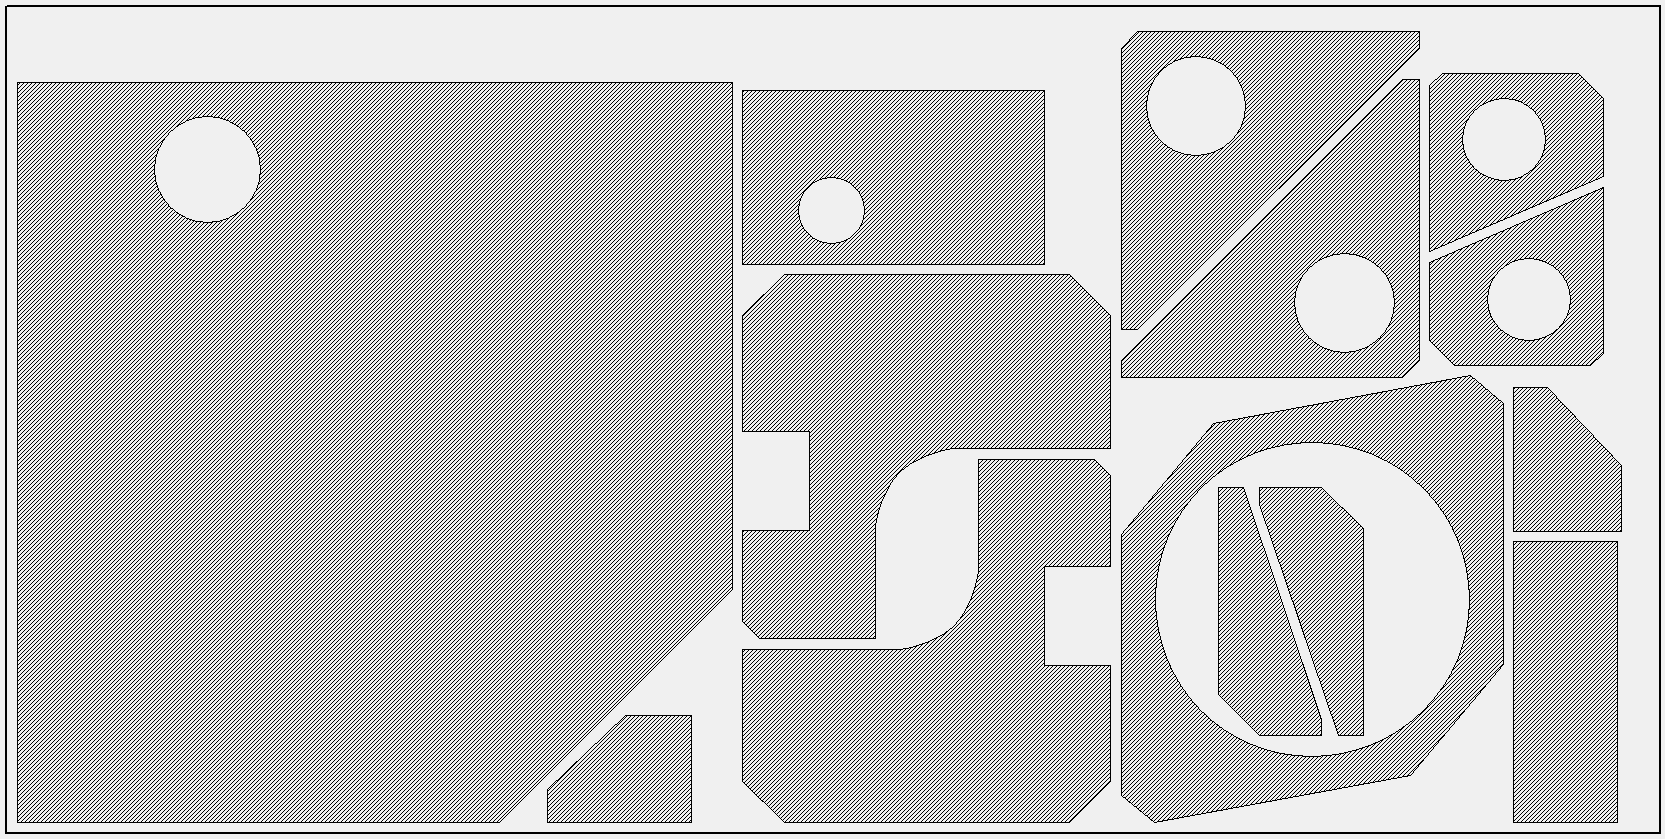
\includegraphics[width=0.9\textwidth]{gsccp-a.png}
    \label{gsccp-a}
  }
  \subfigure[]{
    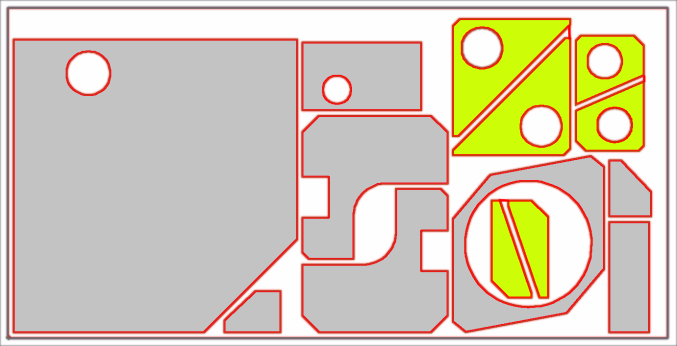
\includegraphics[width=0.9\textwidth]{gsccp-b.png}
    \label{gsccp-b}
  }
  \caption{
    Пример задачи GSCCP с набором из двух комплектов базовых~сегментов: \\
    {\it а} -- 21 базовый сегмент;
    {\it б} -- 18 базовых сегментов
    }
  \label{gsccp-both}
\end{figure}

В качестве целевой функции для данного примера было выбрано
время процесса резки~(\ref{cutting-time}):
$$
  T_{cut} = \frac{L_{on}}{V_{on}} + \frac{L_{off}}{V_{off}} +N_{pt} \cdot t_{pt}
  .
$$

Чтобы свести непрерывные задачи {\it SCCP}
к дискретной модели,
каждый базовый сегмент делится с определенным шагом по точкам,
которые будут претендентами на точку входа инструмента в контур.
Каждая такая точка входа однозначно определяет точку врезки.
В то же время каждая возможная точка врезки должна
удовлетворять технологическим ограничениям процесса резки
(\ref{pierce-constraint}),
то есть многие точки базовых сегментов будут удалены.
Напомним, что для каждого базового сегмента
такая точка может быть только одна.
На рис.~\ref{discrete21}
показано конечное множество возможных точек врезки
для первой задачи
(набор из двадцати одного базового сегмента).
Фактически мы свели первую задачу {\it SCCP}
(в данном конкретном случае эквивалентную {\it CCP})
(рис.~\ref{gsccp-both}, {\it а})
к задаче о последовательном обходе мегаполисов (модели {\it GTSP}).
Обратите внимание,
что в этом случае число возможных маршрутов резки $ROUTE$
становится конечным.
Процесс дискретизации второй задачи SCCP,
рис.~\ref{gsccp-both}, {\it б}
производится аналогичным образом.
Для решения обеих задач применен метод динамического программирования,
использующий специальную схему Беллмана,
которая описана во второй части монографии.

\begin{figure}[H]
  \centering
  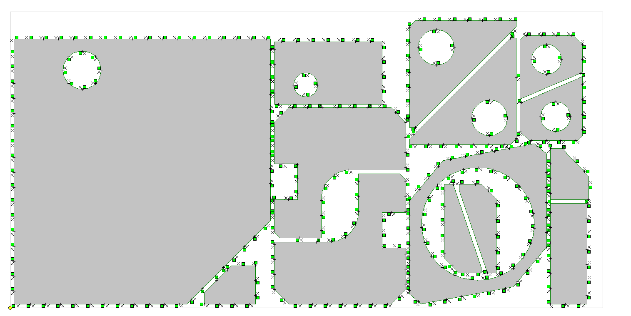
\includegraphics[width=0.9\textwidth]{discrete21.png}
  \caption{
    Дискретизация задачи CCP
    для случая 21 базового сегмента
  }
  \label{discrete21}
\end{figure}

На рис. \ref{gsccp.paths}
показаны оптимальные маршруты резки для двух задач {\it SCCP}
с двацать одним
(рис. \ref{gsccp.paths}, {\it а})
и восемнадцатью
(рис. \ref{gsccp.paths}, {\it б})
базовыми сегментами соответственно.

\begin{figure}[H]
  \centering
  \subfigure[]{
    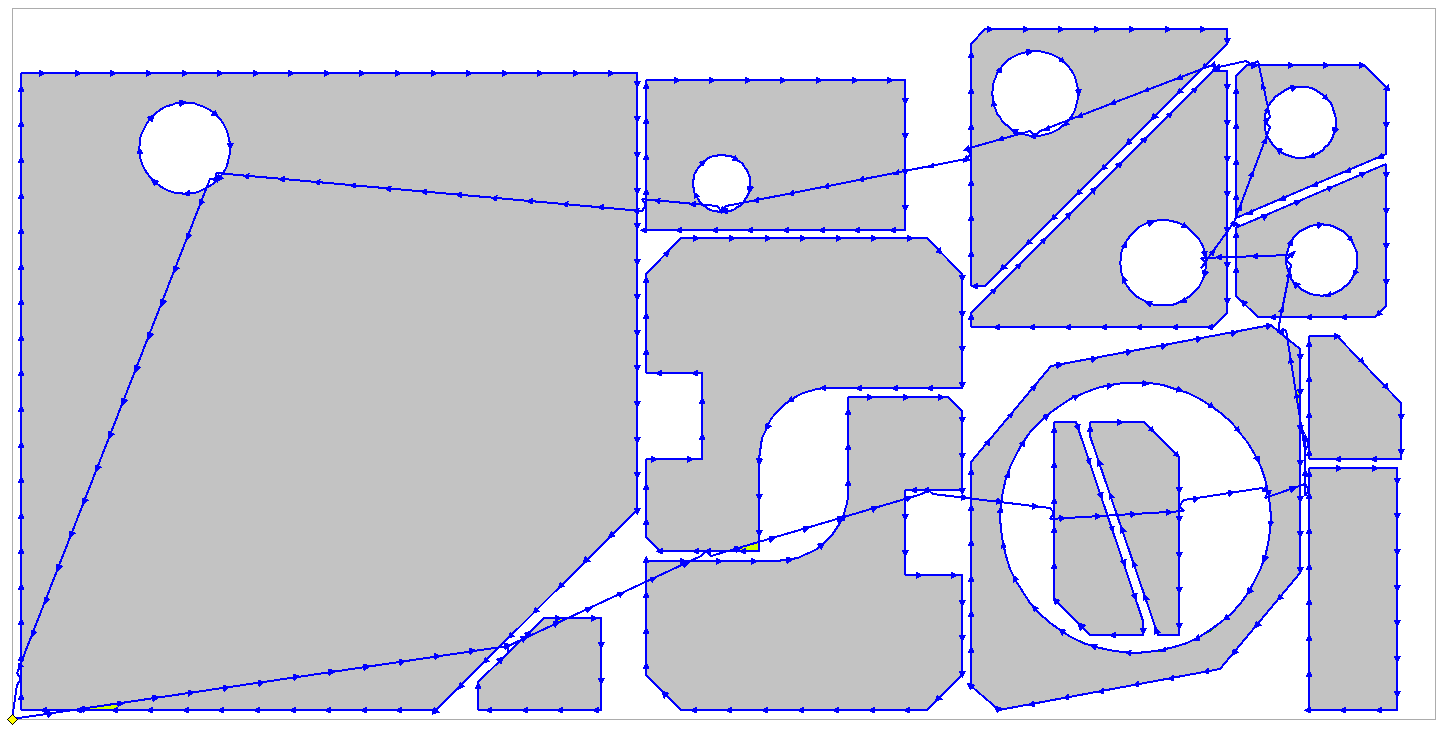
\includegraphics[width=0.9\textwidth]{path21.png}
    \label{path21}
  }
  \subfigure[]{
    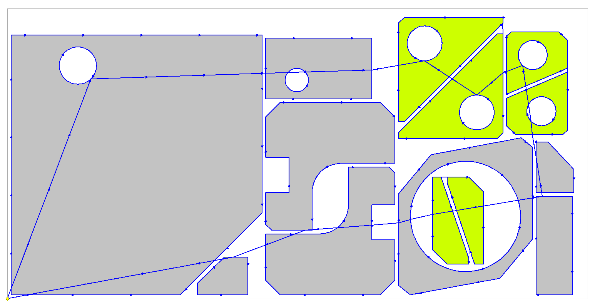
\includegraphics[width=0.9\textwidth]{path18.png}
    \label{path18}
  }
  \caption{
    Схема оптимальной траектории инструмента: \\
    {\it а} -- 21 базовый сегмент;
    {\it б} -- 18 базовых сегментов
  }
  \label{gsccp.paths}
\end{figure}

В первом случае
(21 базовый сегмент)
время процесса резки
$T_{cut}$
составляет 2255 с,
во втором
(18 базовых сегментов)
-- 2244 с.
Обратите внимание, что в первом случае длина рабочего хода инструмента
$L_{on}$
(20567 мм) меньше, чем во втором -- (20727 мм),
но из-за уменьшения количества точек врезки
для восемнадцати сегментов общее время резки также уменьшилось.
Еще раз отметим, что оба решения являются оптимальными
для выбранных наборов базовых сегментов.
Таким образом, оптимальное значение целевой
функции для выбранной задачи {\it GSCCP} составляет 2244 с.

При решении задач были учтены необходимые <<статические>> ограничения:
условия предшествования и ограничения для координат
точек врезки (\ref{pierce-constraint}).
Динамические ограничения в этом модельном примере не рассматривались.

Описанный подход позволяет решать задачи из
наиболее сложного класса задач маршрутизации
траектории инструмента -- {\it ICP},
который не ограничивает выбор точки входа
инструмента в контур детали и использование
любой техники резки.
Наиболее важной особенностью подхода
является возможность для одной задачи оптимизации
формировать разные наборы базовых сегментов и
применять разные алгоритмы оптимизации,
используя как дискретные, так и,
в некоторых случаях, непрерывные модели.
